\documentclass[border=10pt]{standalone}

\usepackage{tikz}
\usepackage{tikzsymbols}
\usetikzlibrary{calc,patterns,shapes.geometric}

\def\centerarc[#1](#2)(#3:#4:#5){\draw[#1] ($(#2)+({#5*cos(#3)},{#5*sin(#3)})$) arc (#3:#4:#5);}

\begin{document}
	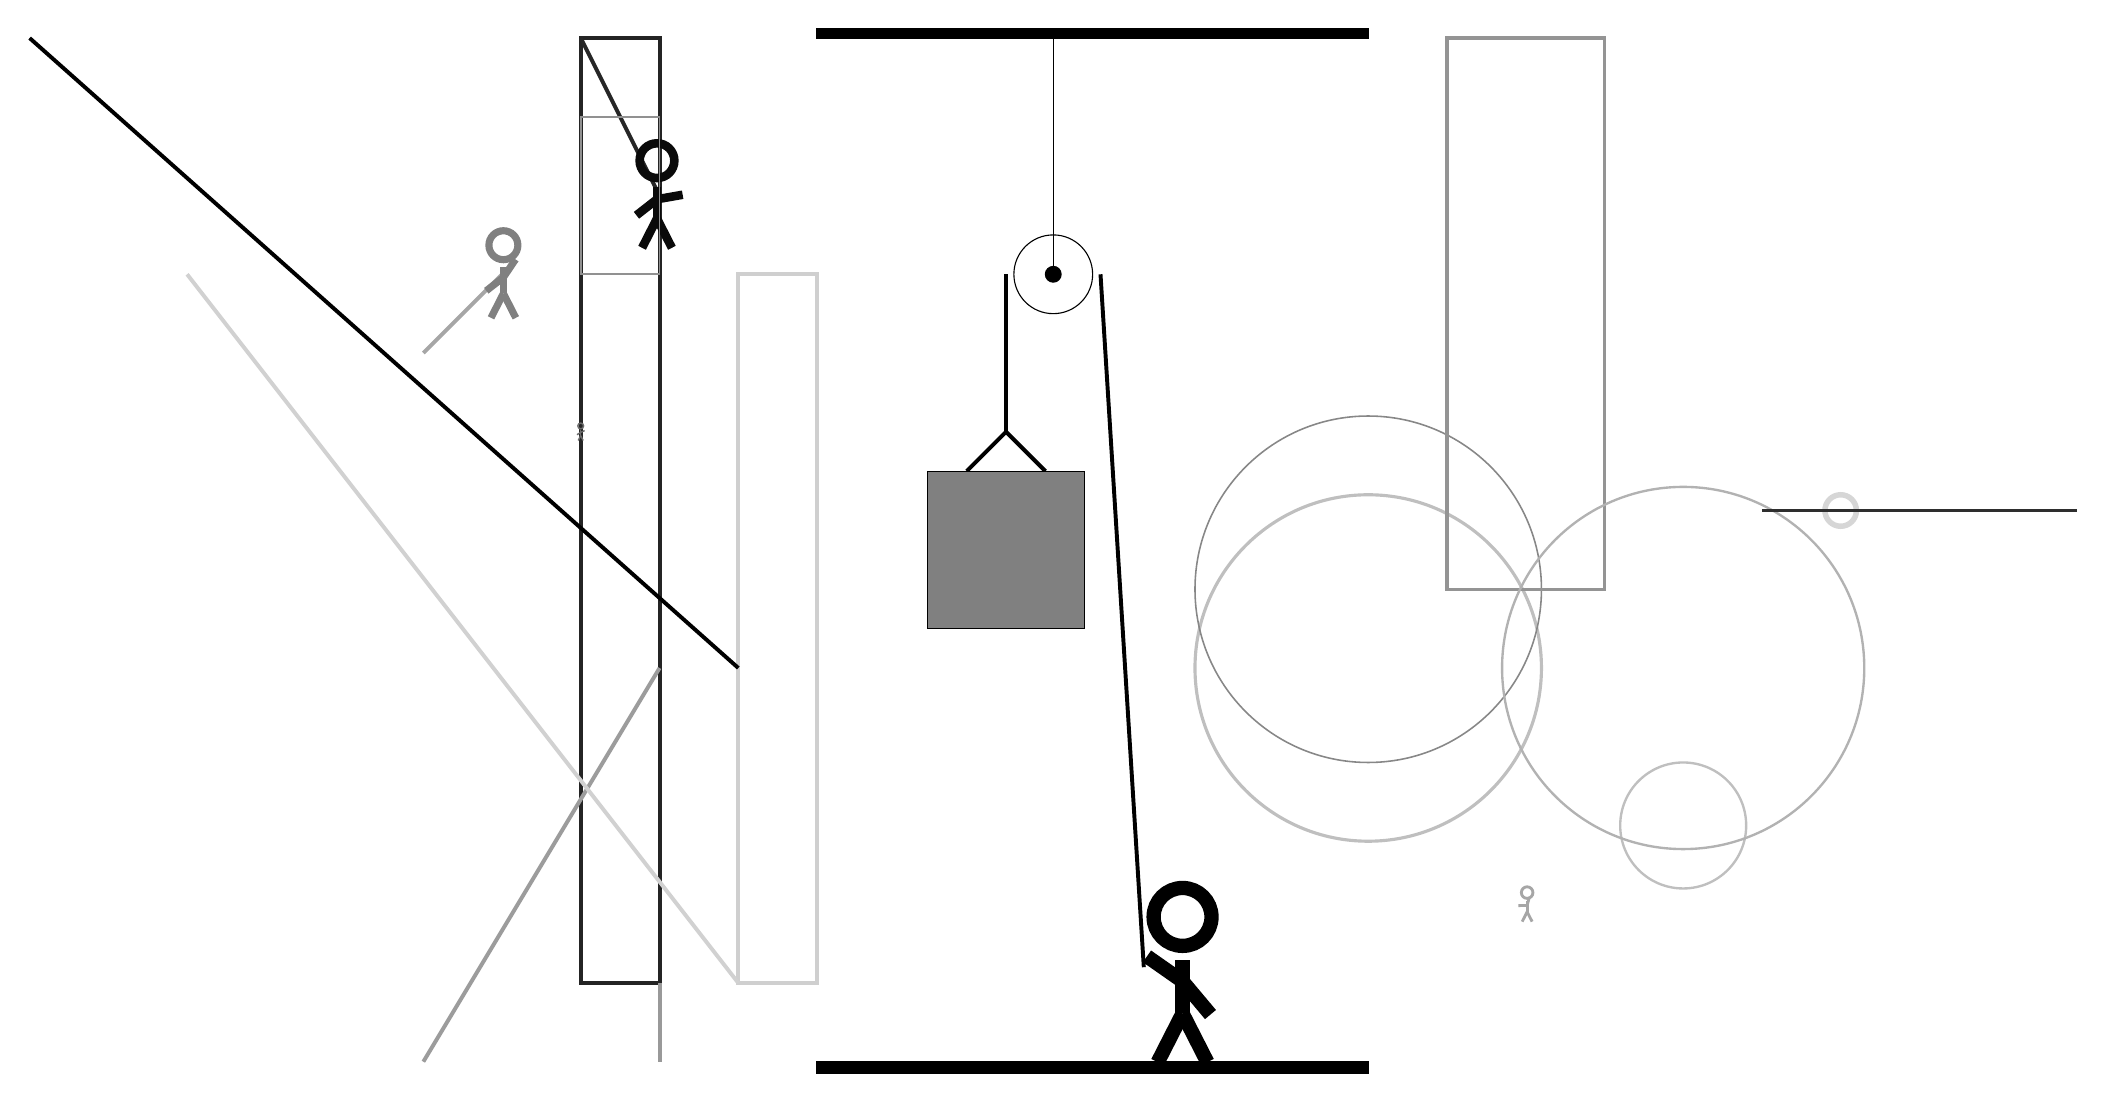
\begin{tikzpicture}
		%%%%% START %%%%%
		
		\draw[fill=black] (-2, 10) rectangle (5, 10.125);
		
		\draw[line width=0.5mm, color=black!86] (-4, 10) rectangle (-5, -2);
		
		\draw [line width=0.5mm, color=black!33](14, -3) circle (0.0);
		\draw [line width=0.4mm, color=black!25](5, 2) circle (2.2);
		\draw[line width=0.5mm, color=black!40](-4, -2) -- (-4, -3);
		
		\draw[line width=0.5mm, color=black!35](-7, 6) -- (-6, 7);
		
		\draw [line width=0.2mm, color=black!47](5, 3) circle (2.2);
		\draw[line width=0.4mm, color=black!42] (6, 3) rectangle (8, 10);
		\draw[line width=0.5mm, color=black!39](-4, 2) -- (-7, -3);
		\draw [line width=0.7mm, color=black!16](11, 4) circle (0.2);
		\draw[line width=0.5mm, color=black!19] (-2, -2) rectangle (-3, 7);
		\node[line width=0.2mm, color=black!50] at (-6, 7) {\Strichmaxerl[5][38][56]};
		\node[line width=0.3mm, color=black!58] at (-5, 5) {\Strichmaxerl[1][32][25]};
		\node[line width=0.3mm, color=black!35] at (7, -1) {\Strichmaxerl[2][1][75]};
		
		\draw[line width=0.5mm, color=black!100](-3, 2) -- (-12, 10);
		\draw[line width=0.5mm, color=black!85](-5, 10) -- (-4, 8);
		\draw [line width=0.3mm, color=black!25](9, 0) circle (0.8);
		
		\node[line width=0.7mm, color=black!96] at (-4, 8) {\Strichmaxerl[6][38][10]};
		\draw [line width=0.3mm, color=black!30](9, 2) circle (2.3);
		\draw[line width=0.5mm, color=black!82](10, 4) -- (14, 4);
		\draw[line width=0.2mm, color=black!43] (-4, 7) rectangle (-5, 9);
		\draw[line width=0.5mm, color=black!18](-3, -2) -- (-10, 7);
		
		
		\draw (1, 7) circle (0.5);
		\draw[fill=black] (1, 7) circle (0.1);
		\draw (1, 10) -- (1, 7);
		
		\draw[line width=0.5mm] (-0.1, 4.5) -- (0.4, 5.0) -- (0.9, 4.5);
		\draw[fill=black!50] (-0.6, 4.5) rectangle (1.4, 2.5);
		
		\draw[line width=0.5mm] (0.4, 7) -- (0.4, 5.0);
		\centerarc[line width=0.5mm](1, 7)(0:180:0.6);
		\draw[line width=0.5mm](1.6, 7) -- (2.15, -1.8);
		
		\node at (2.6, -1.9) {\Strichmaxerl[10][-35][-50]};
		
		\draw[fill=black] (-2, -3) rectangle (5, -3.15);
		
		%%%%% END %%%%%
	\end{tikzpicture}
\end{document}